\documentclass[twoside,11pt]{article}
\PassOptionsToPackage{hyphens}{url}
\usepackage{jmlr2e}
\usepackage{amsmath}
\usepackage[toc,page]{appendix}
\usepackage[table]{xcolor}
\usepackage[marginparsep=30pt]{geometry}
\usepackage{stmaryrd}
\usepackage{algorithm}
\usepackage{algorithmic}
\usepackage{tikz}
\usepackage{tabu}
\usepackage{longtable}
\usepackage{tabularx}
\usepackage{listings}
\usepackage{fancyref}
\usepackage{relsize}
\usepackage{float}
\usepackage{subcaption}

\usetikzlibrary{%
    arrows,
    arrows.meta,
    decorations,
    backgrounds,
    positioning,
    fit,
    petri,
    shadows,
    datavisualization.formats.functions,
    calc,
    shapes,
    shapes.multipart,
    matrix
}

\def\titl{Threaded Programming coursework I: benchmarking
  OpenMP schedules}

\title{\titl}

\author{\name Jonas Fassbender
        \email jonas@fassbender.dev}

\ShortHeadings{\titl}{Jonas Fassbender}
\firstpageno{1}


\begin{document}

\maketitle

\begin{abstract}
\end{abstract}

\begin{keywords}
\end{keywords}

\section{Introduction} % {{{

This paper documents the results of a benchmark performed
on a scientific program.
The program is written in the Fortran programming language
and performs element-wise computations on matrices and
vectors (using nested do-loops, not Fortran's array
operations).
It contains two of these matrix/vector operations---in this
paper called critical sections.

Both critical sections are suitable for speeding up with
OpenMP's loop construct, distributing the computation on
multiple threads of execution.
The loop construct provides the \texttt{schedule} clause,
which determines the division of the loop-iterations
among the OpenMP threads
\citep[see][Chapter 2.7.1]{openmp}.

The benchmark consists of two phases.
The goal of the first phase is to compare different
scheduling options of the OpenMP library and how they
effect the execution speed (measured in seconds) of the two
critical sections of the program.
The second phase provides data on how well the fastest
scheduling options for both critical sections scale with
different amounts of threads.

OpenMP version 4.5 was used and the benchmark was performed
on the back end of the Cirrus supercomputer
\citep[see][]{openmp, cirrus}.
The program was compiled with the Intel Fortran Compiler
(\texttt{ifort}) version 17.0.2, with the maximum
optimization provided (optimization level \texttt{O3})
\citep[see][]{ifort}.

First, this paper describes the conducted benchmark,
before presenting the results. At last the results are
discussed and a conclusion is drawn.

% }}}

\section{Experiment} % {{{
\label{sec:exp}

This chapter will describe the performed benchmark.
First the two critical sections are described
mathematically, followed by a description of the benchmark.

Let $n \in \mathbb{N}$ be a positive integer.
Let $A: n \times n$ and $B: n \times n$ be two matrices,
$A, B \in \mathbb{R}^n \times \mathbb{R}^n$.
Let $A(i, j); 1 \leq i, j \leq n$ be the element of $A$ in
the $i$th row and the $j$th column.
Every element in $A$ is initialized to 0 and every element
in $B$ is set according to:
$B(i, j) = \pi(i+j); i,j=1,\dots,n$.

The first critical section updates $A$:
\begin{align}
  \label{eq:cs1}
  A(i, j) = A(i, j) + \cos(B(i, j)); i,j=1,\dots,n.
\end{align}

Both critical sections are executed multiple times, which
is the reason $A(i, j)$ on the right-hand side of
(\ref{eq:cs1}) can not be substituted to 0.

\def\jmax{\vec{j}_{\text{max} }}

For the second critical section,
let $\vec{c}$ be the zero vector of size $n$.
Let $\jmax \in \mathbb{N}^n$ be another $n$-sized vector.
$\jmax$ is set to:
\begin{align}
  \label{eq:jmax}
  i=1,\dots,n: \jmax(i) =
  \begin{cases}
    n &\text{if } i \text{ mod }
       3\lfloor \frac{i}{30} \rfloor + 1 = 0 \\
    1 &\text{if } i \text{ mod }
       3\lfloor \frac{i}{30} \rfloor + 1 \neq 0
  \end{cases}.
\end{align}
The matrix $B'$ is set to $B'(i, j) = (ij + 1)n^{-2};
i,j = 1,\dots,n$.

The second critical section updates $\vec{c}$:
\begin{align}
  \label{eq:cs2}
  \vec{c}(i) = \sum_{j=1}^{\jmax(i)}\sum_{k=1}^{j}
    \vec{c}(i) + k\ln(B'(j, i))n^{-2}, i=1,\dots,n.
\end{align}

Since both (\ref{eq:cs1}) and (\ref{eq:cs2}) are
element-wise independent, the computation of every element
can be distributed over multiple processes.

It should be noted here, that (\ref{eq:cs1}) is a perfect
computational cube of $n \times n$.
That means, that every iteration---each a manipulation
of a single cell $A(i, j)$---contains the same amount of
instructions, making it trivial to split the iterations
and having a balanced distribution of work per thread.

On the other hand one can see that (\ref{eq:cs2}) does not
behave in the same way.
Each iteration is dependent on $\jmax(i)$, which is not
constant.
Instead, $\jmax(i)$ equals either 1 or $n$ and the
distribution of $\jmax(i) = n$ is asymmetric, since
the modulus in (\ref{eq:jmax}) changes depending on the
iteration $i$.
For example, $\jmax(i) = n$ for every element in the
interval $i \in (1, 29)$, while $\jmax(i) = n$ is true for
only 7 elements in $i \in (30, 59)$ and the amount keeps
decreasing with bigger $i$.
This has the consequence, that the first iterations are
computationally more heavy and time consuming than
the later iterations.

The benchmark consists of two phases.
In the first phase, different scheduling options are
compared using four threads and the fastest scheduling
option for each critical section is determined.
The second part of the benchmark tests how well the
fastest scheduling options scale with different amounts of
threads.
For the benchmark $n$ was set to 729.

The different scheduling options used in the first phase
are:
\begin{itemize}
  \item Auto
  \item Static
  \item Static, Dynamic, Guided, all with different
    chunk sizes of: 1, 2, 4, 8, 16, 32, 64
\end{itemize}

The fastest scheduling options for the critical sections
are then run with 1, 2, 4, 6, 8, 12 and 16 threads during
the second phase of the benchmark.

Like stated in the introduction, both benchmark phases are
executed on the Cirrus back end with exclusive access to one
node.
Every scheduling option in phase one and every amount of
threads in phase two were executed 100 times and the
average and median walltime---in seconds---were measured
with the timing routine \texttt{omp\_get\_wtime}, provided
by OpenMP \citep[see][Chapter 3.4.1]{openmp}.
The average walltime was used as the decisive criteria for
execution speed.
The mean was used as the secondary criteria.

% }}}

\section{Results} % {{{

% phase one fig, table {{{
\begin{table}
\begin{center}
\begin{tabu}{l|ll|ll}
schedule &\multicolumn{2}{l|}{critical section 1}
         &\multicolumn{2}{l}{critical section 2} \\
\hline
&mean &median &mean &median \\
\hline
Sequential&1.62 &1.61 &8.57 &8.56\\
Auto&0.49 &0.48 &5.32 &5.32\\
Static&0.83 &0.84 &6.18 &6.19\\
Dynamic, 1&0.51 &0.51 &2.68 &2.57\\
Dynamic, 2&0.50 &0.49 &2.65 &2.57\\
Dynamic, 4&0.49 &0.49 &2.43 &2.39\\
Dynamic, 8&0.49 &0.48 &\textbf{2.22} &\textbf{2.22}\\
Dynamic, 16&\textbf{0.48} &\textbf{0.48} &2.23 &2.23\\
Dynamic, 32&0.49 &0.48 &3.91 &3.91\\
Dynamic, 64&0.52 &0.51 &4.81 &4.81\\
Guided, 1&0.49 &0.49 &5.33 &5.34\\
Guided, 2&0.49 &0.48 &5.33 &5.33\\
Guided, 4&0.49 &0.49 &5.33 &5.33\\
Guided, 8&0.49 &0.48 &5.33 &5.33\\
Guided, 16&0.49 &0.48 &5.33 &5.33\\
Guided, 32&0.50 &0.49 &5.33 &5.33\\
Guided, 64&0.50 &0.49 &5.33 &5.33\\
Static, 1&0.53 &0.53 &3.96 &3.93\\
Static, 2&0.51 &0.51 &2.84 &2.81\\
Static, 4&0.52 &0.52 &2.60 &2.57\\
Static, 8&0.52 &0.52 &2.37 &2.37\\
Static, 16&0.54 &0.53 &3.17 &3.18\\
Static, 32&0.56 &0.56 &4.84 &4.84\\
Static, 64&0.62 &0.63 &5.37 &5.38\\
\end{tabu}

\caption{Results of phase one of the benchmark. Displayed
  are average and median walltime in seconds for every
  scheduling option for both critical sections. The fastest
  scheduling options are marked with a bold font-weight.}
\label{tab:p1}
\end{center}
\end{table}

\begin{figure}
\begin{subfigure}{\textwidth}
\begin{center}
% critical section 1 {{{
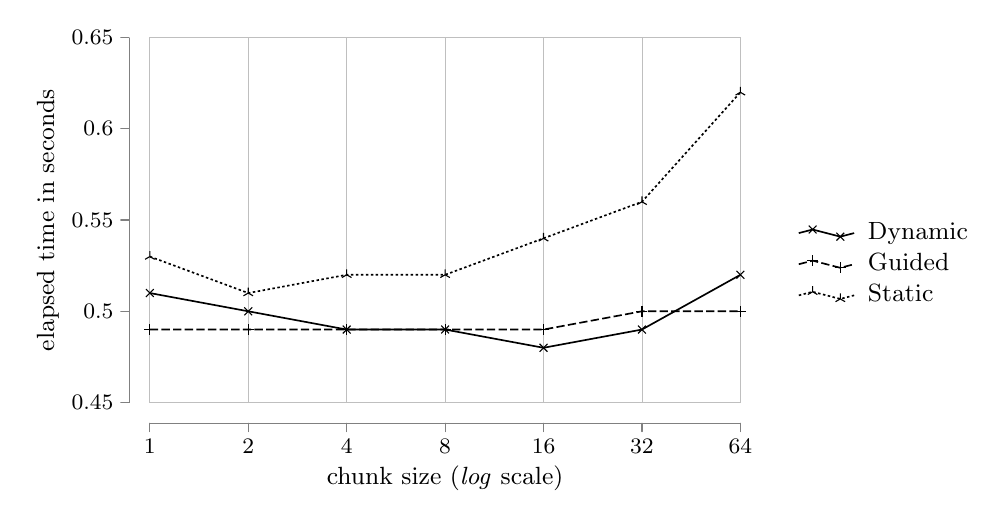
\begin{tikzpicture}[scale=1.5]
  \datavisualization[
    scientific axes=clean,
    visualize as line/.list={dynamic,guided, static},
    style sheet=vary dashing,
    style sheet=cross marks,
    dynamic={label in legend={text=Dynamic}},
    guided={label in legend={text=Guided}},
    static={label in legend={text=Static}},
    x axis={
      logarithmic,
      ticks={major={at={1,2,4,8,16,32,64} } },
      label={chunk size (\textit{log} scale)},
      grid={minor={at={2,4,8,16,32} }},
    },
    y axis={
      include value={0.45, 0.65},
      label={elapsed time in seconds},
    },
  ]
  data[set=dynamic]{
    x,  y
    1,  0.51
    2,  0.50
    4,  0.49
    8,  0.49
    16, 0.48
    32, 0.49
    64, 0.52
  }
  data[set=guided]{
    x,  y
    1,  0.49
    2,  0.49
    4,  0.49
    8,  0.49
    16, 0.49
    32, 0.50
    64, 0.50
  }
  data[set=static]{
    x,  y
    1,  0.53
    2,  0.51
    4,  0.52
    8,  0.52
    16, 0.54
    32, 0.56
    64, 0.62
  };
\end{tikzpicture}
% }}}
\caption{Critical section 1.}
\end{center}
\vspace{0.5cm}
\end{subfigure}
\begin{subfigure}{\textwidth}
\begin{center}
% critical section 2 {{{
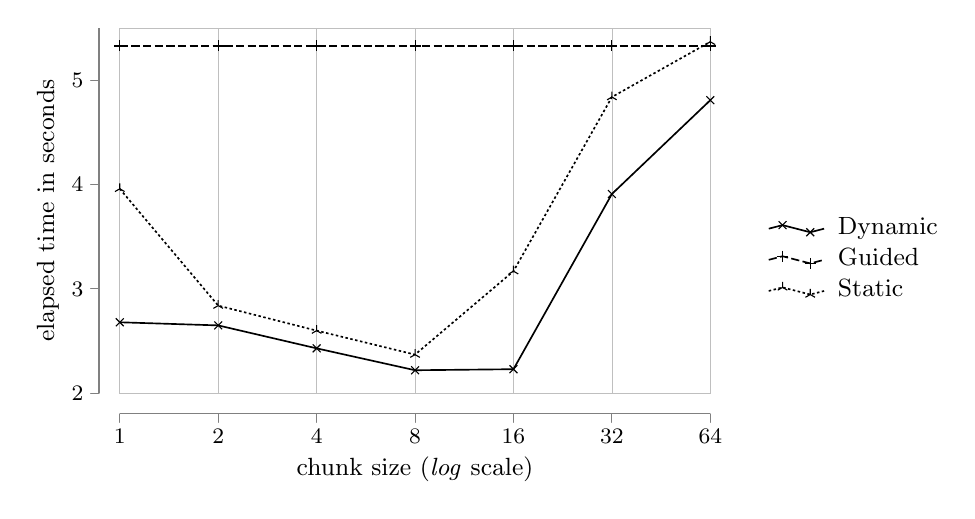
\begin{tikzpicture}[scale=1.5]
  \datavisualization[
    scientific axes=clean,
    visualize as line/.list={dynamic,guided, static},
    style sheet=vary dashing,
    style sheet=cross marks,
    dynamic={label in legend={text=Dynamic}},
    guided={label in legend={text=Guided}},
    static={label in legend={text=Static}},
    x axis={
      logarithmic,
      ticks={major={at={1,2,4,8,16,32,64 } } },
      label={chunk size (\textit{log} scale)},
      grid={minor={at={2,4,8,16,32} }},
    },
    y axis={
      include value={2, 5.5},
      label={elapsed time in seconds},
    },
  ]
  data[set=dynamic]{
    x,  y
    1,  2.68
    2,  2.65
    4,  2.43
    8,  2.22
    16, 2.23
    32, 3.91
    64, 4.81
  }
  data[set=guided]{
    x,  y
    1,  5.33
    2,  5.33
    4,  5.33
    8,  5.33
    16, 5.33
    32, 5.33
    64, 5.33
  }
  data[set=static]{
    x,  y
    1,  3.96
    2,  2.84
    4,  2.60
    8,  2.37
    16, 3.17
    32, 4.84
    64, 5.37
  };
\end{tikzpicture}
% }}}
\caption{Critical section 2.}
\end{center}
\vspace{0.5cm}
\end{subfigure}
\caption{Plots on how the chunk size clause changes the
  execution speed of the Dynamic, Guided and Static
  scheduling options, for both critical sections.}
\label{fig:chunk_size}
\end{figure}
% }}}

Table~\ref{tab:p1} lists the average and median
walltime in seconds for the execution of the critical
sections, determined in phase one of the benchmark.

Sequential is not a schedule. It represents execution time
of the critical section in a sequential, not parallelized
manner.

One can see, that for the first---the symmetric---critical
section the schedules do not differentiate much concerning
the execution time.
Especially the Auto, Dynamic, $n$ and Guided, $n$
scheduling options are all between $0.48$ and $0.52$
seconds of average execution time.
Static, $n$ performs slightly worse, all options having
an average execution time between $0.51$ and $0.56$
seconds, except Static, 64, which performs worse with an
average execution time of 0.62 seconds.
The Static scheduling option, which just splits the
iterations in \#threads (in this case four) approximately
equal chunks, performs the worst with an average execution
time of 0.83 seconds \citep[see][]{lecture}.

The best scheduling option for the first critical section
is Dynamic, 16, with an average and median execution time
of 0.48 seconds.

The schedules differ much more in execution time for
the second critical section, compared to the first one.

The difference between Dynamic, 8 (fastest) and Static
(slowest) is nearly 4 seconds, which makes Static
approximately 2.8 times slower than Dynamic, 8.
For comparison, the slowest scheduling option for
the first critical section is just approximately 1.7 times
slower than the fastest scheduling option.

Guided, $n$ and Auto, which were close to fastest in
the first critical section, perform worse on the
section critical section. All are approximately 2.4 times
slower than Dynamic, 8.

Static, $n$ fluctuates the most with different chunk
size $n$.
Static, 8, with 2.37 seconds average execution time, is
the third fastest scheduling option, while Static, 64
is the second slowest scheduling option with 5.37 seconds
average execution time.

The fluctuation of the average execution time, based
on different chunk sizes can be seen in
Figure~\ref{fig:chunk_size}.

During the second phase of the benchmark the two scheduling
options resulting in the fastest average execution time
were tested with different amounts of threads.
The fastest scheduling option for the first critical
section was Dynamic, 16. For the second critical section
Dynamic, 8 resulted in the fastest average execution time.

Table~\ref{tab:p2} lists the average and median execution
time in seconds for both scheduling options when run
with 1, 2, 4, 6, 8, 12 and 16 threads.

Figure~\ref{fig:speedup} displays how much using more
threads gains in exectution speed, compared to using just
one thread (sequential execution).
While for the first critical section the speedup of using
more threads grows linear, the execution time for the
second critical section stops being faster after 6
threads (see Table~\ref{tab:p2}, Figure~\ref{fig:speedup}).

% phase two fig, table {{{
\begin{table}
\begin{center}
\begin{tabu}{ll|XXXXXXX}
\#threads & &1 &2 &4 &6 &8 &12 &16 \\
\hline
loop 1 &mean &1.87 &0.94 &0.48 &0.34 &0.26 &0.19 &0.15 \\
       &median &1.87 &0.93 &0.48 &0.34 &0.26 &0.18 &0.14 \\
\hline
loop 2 &mean &8.59 &4.30 &2.22 &2.08 &2.09 &2.08 &2.07 \\
       &median &8.59 &4.30 &2.22 &2.08 &2.10 &2.08 &2.07 \\
\end{tabu}

\caption{Results of phase two of the benchmark. Displayed
  are average and median walltime in seconds for the
  fastest scheduling options from phase one, for each
  critical section, executed with different amounts of
  threads.}
\label{tab:p2}
\end{center}
\end{table}

\begin{figure}
\begin{subfigure}{\textwidth}
\begin{center}
% critical section 1 {{{
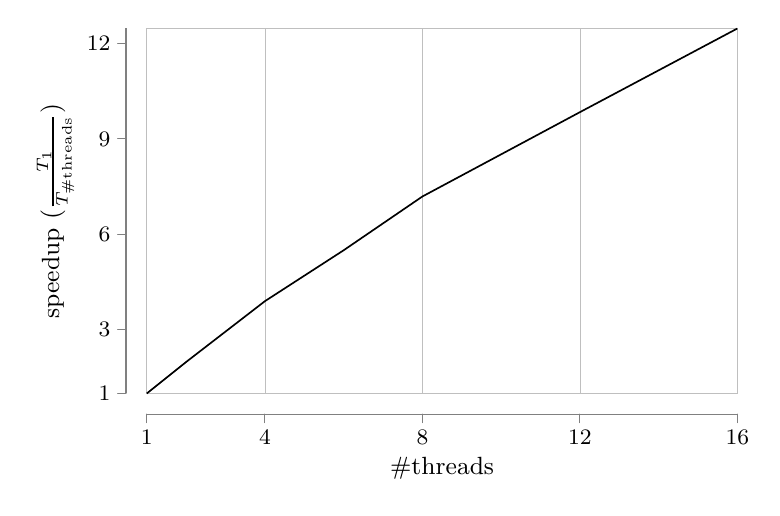
\begin{tikzpicture}[scale=1.5]
  \datavisualization[
    scientific axes=clean,
    visualize as line,
    x axis={
      ticks={major={at={1,4,8,12,16}} },
      label={\#threads},
      grid={minor={at={4,8,12} }},
    },
    y axis={
      ticks={major={at={1,3,6,9,12}} },
      label={speedup ($\frac{T_1}{T_{\text{\#threads}} }$)},
    }
  ]
  data{
    x,  y
    1,  1
    2,  1.99
    4,  3.90
    6,  5.50
    8,  7.19
    12, 9.84
    16, 12.47
  };
\end{tikzpicture}
% }}}
\caption{Critical section 1.}
\end{center}
\vspace{0.5cm}
\end{subfigure}

\begin{subfigure}{\textwidth}
\begin{center}
% critical section 2 {{{
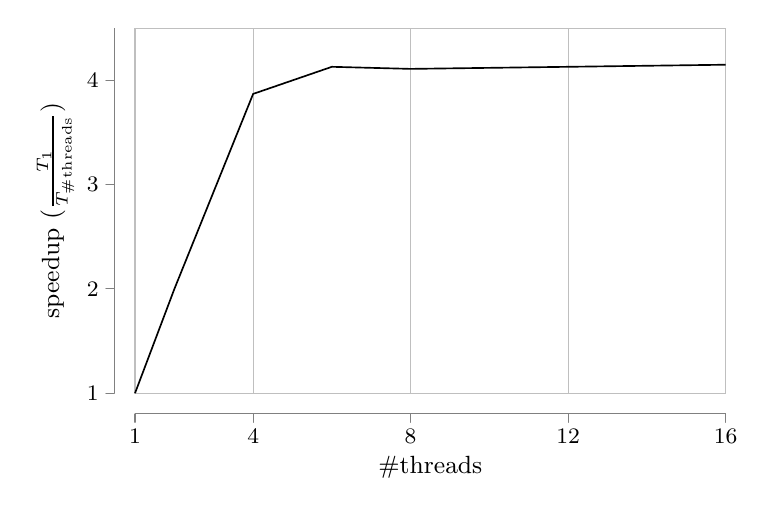
\begin{tikzpicture}[scale=1.5]
  \datavisualization[
    scientific axes=clean,
    visualize as line,
    x axis={
      ticks={major={at={1,4,8,12,16}} },
      label={\#threads},
      grid={minor={at={4,8,12} }},
    },
    y axis={
      include value={1,4.5},
      label={speedup ($\frac{T_1}{T_{\text{\#threads}} }$)},
    }
  ]
  data{
    x,  y
    1,  1
    2,  2.00
    4,  3.87
    6,  4.13
    8,  4.11
    12, 4.13
    16, 4.15
  };
\end{tikzpicture}
% }}}
\caption{Critical section 2.}
\end{center}
\vspace{0.5cm}
\end{subfigure}
\caption{Plots on how the execution speed varies with the
  amount of threads. The plots show how much faster more
  threads are, compared to just one thread.}
\label{fig:speedup}
\end{figure}
% }}}

% }}}

\section{Discussion}

There are several statements to make about why some
scheduling options outperform each other.

For the first critical section only Static and Static, $n$
perform worse than the others.
Guided, $n$ has approximately the same performance
as Dynamic, $n$ (also it is more constant with different
chunk sizes). This suggests, that the reason why Static and
Static, $n$ perform worse must lie in the later iterations.
This could have two reasons: (\romannumeral 1) longer
indexing of $B(i, j)$; (\romannumeral 2) $\cos(x)$ takes
longer to compute for bigger $x$
(see Equation~\ref{eq:cs1}).
Problem (\romannumeral 2) could easily be solved by
setting $B(i, j) = B(i, j) \mod 2\pi$, since if
$x \equiv y (\text{mod }2\pi)$, then $\cos(x) = \cos(y)$
(follows from the fact that $\cos(x)$ has $2\pi$ as its
period) \citep[see e.g.][]{trig}.

% here results for second critical section

% first iter now worse than last => guided sucks, big static sucks
% auto can not adopt

% big n suck for both, since iterations are so asymmetrical
% small n suck in general, because switching overhead

% phase 2: why tf does cs2 not scale


\section{Conclusion}

% even though cs1 looks symmetric, for big values it gets
% worse



\bibliography{tpcw.bib}

\end{document}
